\newcommand{\uL}{\mathbf{L_0}}
\newcommand{\bL}{\mathbf{\bar{L}_0}}
\begin{frame}{Level identification in CFT spectra}
\vskip-1.5cm
\only<1>{

To make a precise comparison with the free-boson CFT, we'll need to solve for (or look up) the solution of this model.

The free-boson CFT is created from the Lagrangian 
$$ \mathfrak{L} = \frac{g}{2}\int dt \int\limits_0^L dx ( \frac{1}{v^2}(\partial_t \phi)^2 - (\partial_x \phi)^2)$$
and with the compatified field identification
$$ \phi \equiv \phi + 2\pi R$$
and placed on the circle of circumference $L$ with periodic boundary conditions
$$ \phi(x) \equiv \phi(x+L).$$
}
\only<2>{
\begin{table}[h]
\centering
\begin{tabular}{c|c}
$\uL$ & $2\pi g(\frac{e}{4 \pi g R} + \frac{m R}{2})^2 + n$  \\
& \\
$\bL$ & $2\pi g(\frac{e}{4 \pi g R} - \frac{m R}{2})^2 + \bar{n}$  \\
& \\
$\mathbf{P} =\frac{2\pi v}{L}(\uL-\bL)$ & $\frac{2\pi v}{L}(em + n - \bar{n})$ \\
& \\
$\mathbf{H} = \frac{2\pi v}{L}(\uL+\bL)$ & $\frac{2\pi v}{L}(\frac{e^2}{4 \pi g R^2} + \pi g m^2 R^2 + n + \bar{n})$ \\
& \\
$\tilde{\mathbf{H}} = \frac{L}{2 \pi v \kappa}\mathbf{H}$ & $e^2 + \frac{m^2}{4 \kappa^2} + \frac{1}{\kappa}(n + \bar{n})$       
\end{tabular}
\label{Table:EV}
\caption{Eigenvalues of states $\ket{e, m}_{n, \bar{n}}$. The rescaled Hamiltonian $\tilde{\mathbf{H}}$ has eigenvalues that depend on only one free-parameter, $\kappa = 1/(4 \pi g R^2)$.(Note: A common convention is to set $g=1/4\pi$ and describe the system using $R=\sqrt{1/\kappa}$.) }
\end{table}
}
\only<3->{
\begin{figure}[hbctp]
\begin{center}
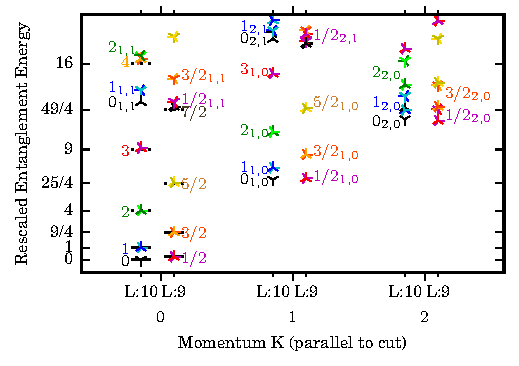
\includegraphics[height=\textheight]{{interpolatedboson/a10/plots/EEIdentify.pdf}}
\end{center}
%\caption{The identification of the states $\ket{e, m}_{n, \bar{n}}$ in the spectrum of the soft-core boson entanglement Hamiltonian. The label $e$ gives the U(1) charge. The labels $n$, $\bar{n}$ label the levels in the right or left-moving sectors of the Kac-Moody algebra. When the level $n$ is larger than 1, the level shows $Z(n)$ approximately degenerate states. The best estimate for the Luttinger parameter $\kappa = 1/6.4$ is given by the inverse of the energy of the $\ket{1, 0}_{1, 0}$ state. The label $m$ is 0 for all states shown - however, the primary states $\ket{e, m=\pm 1}$ can be seen centered around momentum $\pi$, with energies on the order of $1/(4\kappa^2)$.}
%\label{fig:primaries}
\end{figure}
}  
\end{frame}